% --- SLIDE 2: The Data Deluge \ Memory Bottleneck ---
% \begin{frame}{The Memory Bottleneck}
%     \framesubtitle{Why Space Efficiency Matters}
%     \begin{block}{Data is Exploding}
%         Massive datasets from Science, Web, AI, IoT... (Petabytes, Exabytes). Fast analysis needs data in Main Memory (RAM).
%     \end{block}
%     \pause % Step 1
%     \begin{alertblock}{The Bottleneck: RAM vs. Storage}
%         \begin{itemize}
%             \item RAM: \alert{Fast}, but \alert{Small} (GBs).
%             \item Disk/Cloud: \alert{Slow}, but \alert{Huge} (TBs/PBs).
%             \item Speed Difference: Factor of $\sim \mathbf{10^5}$!
%         \end{itemize}
%     \end{alertblock}
%     \pause % Step 3
%     \begin{block}{The Structure Overhead Problem}
%         Often, the \emph{auxiliary data structure} (index, tree, etc.) needed for queries is \textbf{much larger} than the data itself.
%         \vspace{0.5em}
%         $\implies$ Fitting data + structures in RAM is hard.
%     \end{block}
% \end{frame}

% % --- SLIDE 3: The Promise of Succinct Data Structures ---
% \begin{frame}{The Promise of Succinct Data Structures}
%     \framesubtitle{Getting the Best of Both Worlds}
%     We face a classic trade-off:
%     \begin{columns}[T]
%         % Colonna Sinistra: Compression
%         \begin{column}{0.5\textwidth}
%             \begin{block}{Standard Compression}
%                 \centering
%                 \textbf{Pro:} \alert{Minimal Space} \\
%                 \textbf{Con:} Slow / No Direct Queries
%             \end{block}
%         \end{column}
%         \begin{column}{0.5\textwidth}
%             \begin{block}{Traditional Data Structures}
%                 \centering
%                 \textbf{Pro:} \alert{Fast Queries} \\
%                 \textbf{Con:} Often Large Space Overhead
%             \end{block}
%         \end{column}
%     \end{columns}
%     % Introduce Succinct goal
%     \begin{alertblock}<2->{The Succinct Goal}
%         Can we achieve \textbf{both} simultaneously?
%         \begin{itemize}
%             \item Space usage \alert{close to the information-theoretic lower bound} of the data.
%             \item Support efficient queries \alert{directly} on this compact representation.
%         \end{itemize}
%     \end{alertblock}
% \end{frame}

% --- SLIDE 2 (Combined): The Need for Space Efficiency & Succinct Structures ---
\begin{frame}{Why Succinct Data Structures?}
    \framesubtitle{Massive Data and Structure Overhead}

    \begin{block}<1->{The Challenge: Massive Data \& Query Needs}
        Modern datasets (Science, Web, AI...) are enormous.
        Complex analysis demands data in RAM, but auxiliary structures (indexes, trees) needed for queries often \textbf{occupy more space than the data itself}.
        $\implies$ Fitting everything in RAM is a major bottleneck.
    \end{block}

    \begin{columns}[T]
        \begin{column}<2->{0.45\textwidth}
            \textbf{Classic Trade-off:}
            \begin{itemize}
                \item \textit{Compression:} Minimal space, but slow/no direct queries.
                \item \textit{Traditional Data Structures:} Fast queries, but large space overhead.
            \end{itemize}
        \end{column}
        \begin{column}<3->{0.55\textwidth}
            \begin{alertblock}{The Succinct Goal: Best of Both Worlds}
                Can we achieve \textbf{both}?
                \begin{itemize}
                    \item Space \alert{near information-theoretic minimum}.
                    \item Efficient queries \alert{directly} on compact data.
                \end{itemize}
            \end{alertblock}
        \end{column}
    \end{columns}
\end{frame}

% \begin{frame}{Standard Compression vs. Succinct Data Structures}
%     \framesubtitle{Accessing Compressed Data}
%     \begin{figure}[htbp]
%         \centering
%         \only<1>{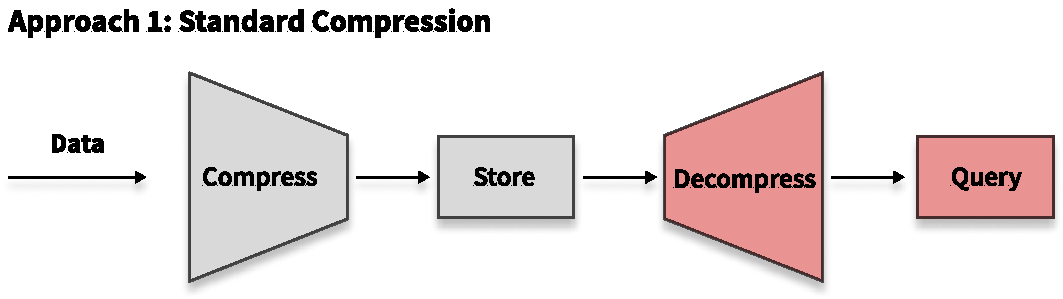
\includegraphics[width=0.8\textwidth]{assets/succint-pipeline1.pdf}}
%         \only<2>{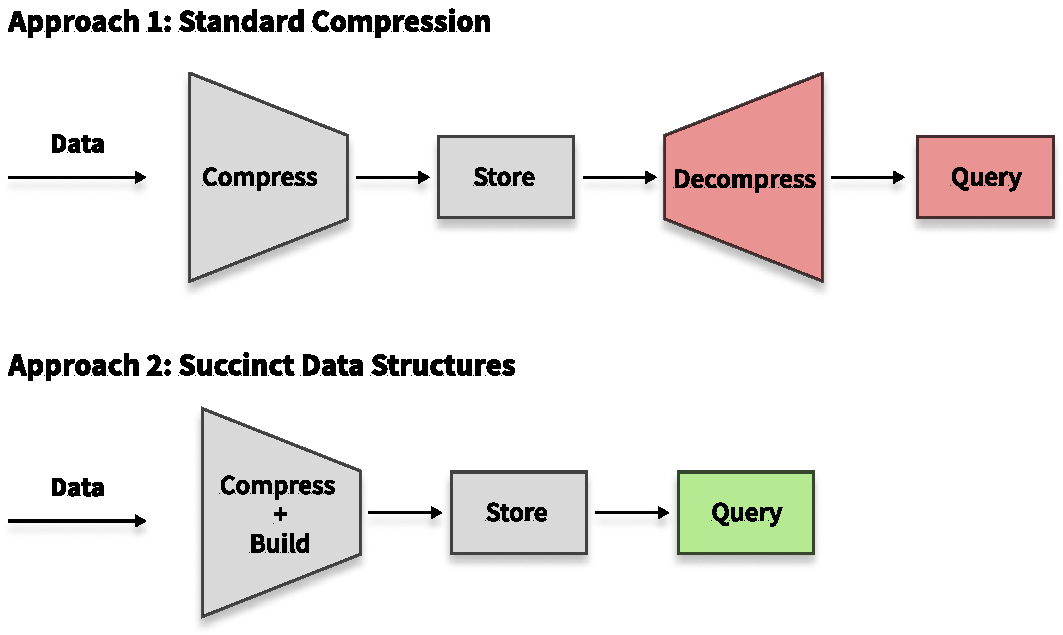
\includegraphics[width=0.8\textwidth]{assets/succint-pipeline.pdf}}
%     \end{figure}
% \end{frame}

% \begin{frame}{Information Theory \& Compression Limits}
%     \framesubtitle{The Role of Probability}
%     Consider a data source modeled as a random variable $X$ taking values in $\mathcal{X}$. \newline
%     \textbf{Question:} What is the minimum \emph{average} number of bits per symbol needed for a lossless representation of $X$?
%     \begin{alertblock}{Fundamental Insight (Shannon)}
%         The answer depends intrinsically on the \textbf{probability distribution} $P_X(x) = \text{Pr}\{X=x\}$.
%     \end{alertblock}
%     \begin{itemize}
%         \item<2-> Uniform Distribution ($P_X(x) = 1/|\mathcal{X}|$): High uncertainty. Requires $\approx \log_2 |\mathcal{X}|$ bits/symbol.
%         \item<3-> Non-Uniform Distribution: Lower average uncertainty. Allows for compression by assigning shorter codes to more probable symbols.
%     \end{itemize}
%     \uncover<4->{We need a precise measure of this "average uncertainty"...}
% \end{frame}

% \begin{frame}{Shannon Entropy: The Lower Bound}
%     \framesubtitle{Quantifying Average Information}
%     \begin{definition}[Shannon Entropy $H(X)$]
%         The average uncertainty (information content) of source $X$ with distribution $P_X$:
%         \[ H(X) = E_{P_X}[-\log_2 P_X(x)] = -\sum_{x \in \mathcal{X}} P_X(x) \log_2 P_X(x) \quad [\text{bits/symbol}] \] % Units in brackets
%     \end{definition}
%     \begin{alertblock}{Fundamental Result (Shannon)} % Changed title from Theorem
%         The Shannon Entropy $H(X)$ establishes the theoretical \textbf{minimum average number of bits per symbol} required to represent the output of source $X$ without loss of information.
%         \vspace{0.5em} % Small space inside block
%         \\ No representation can achieve, on average, fewer than $H(X)$ bits per symbol.
%     \end{alertblock}
%     $\implies$ $H(X)$ is the ultimate benchmark for space efficiency that Succinct Data Structures aim to approach.
% \end{frame}

% --- SLIDE 4: Information Theory and Shannon Entropy ---
\begin{frame}{Shannon Entropy}
    \framesubtitle{Fundamental Limits of Lossless Compression}

    % Passo 1: Obiettivo
    \textbf{Goal:} Determine the minimum average number of bits per symbol required for a lossless representation of data from a source $X$.
    \pause % Pausa 1

    % % Passo 2: Principio Fondamentale
    % \begin{block}{Fundamental Principle (Shannon, 1948)}
    %     This minimum is intrinsically linked to the source's \textbf{probability distribution} $P_X(x) = \text{Pr}\{X=x\}$.
    %     % Non-uniform distributions imply lower average uncertainty and allow for greater compression compared to uniform distributions ($\approx \log_2 |\mathcal{X}|$ bits/symbol).
    % \end{block}
    % \pause % Pausa 2

    % Passo 3: Definizione dell'Entropia
    % The measure quantifying this average information content is the \emph{Shannon Entropy}:
    % \vspace{0.5em} % Piccolo spazio
    \begin{definition}[Shannon Entropy $H(X)$]
        The average uncertainty, or information content, per symbol of source $X$:
        \[ H(X) = E_{P_X}[-\log_2 P_X(x)] = -\sum_{x \in \mathcal{X}} P_X(x) \log_2 P_X(x) \quad [\text{bits/symbol}] \]
    \end{definition}
    \pause % Pausa 3

    % Passo 4: Teorema del Limite Inferiore e Rilevanza
    \begin{alertblock}{Source Coding Theorem (Lower Bound)}
        Shannon proved that $H(X)$ constitutes the \textbf{theoretical lower bound} on the average number of bits per symbol required to represent the output of source $X$ without loss of information.
    \end{alertblock}

    % \uncover<5->{
    %     $\implies$ $H(X)$ serves as the fundamental benchmark for evaluating the space efficiency of data representations, including Succinct Data Structures.
    % }

\end{frame}

% --- SLIDE 5: Zero-Order Empirical Entropy ---
\begin{frame}{Zero-Order Empirical Entropy}
    \framesubtitle{A Practical Bound Based on Data}
    We usually don't know the true source $P_X$. We only have the data sequence $S$.
    \pause
    \begin{definition}[Zero-Order Empirical Entropy $\mathcal{H}_0(S)$]
        Information content of sequence $S$ based on its symbol counts ($n_s$):
        \[ \mathcal{H}_0(S) = \sum_{s \in \Sigma} \frac{n_s}{n} \log_2 \frac{n}{n_s} \quad [\text{bits/symbol}] \]
        Uses observed frequencies $\frac{n_s}{n}$ instead of unknown $P_X(x)$.
    \end{definition}
    \pause
    \begin{alertblock}{Relevance for Succinct Structures}
        $n \cdot \mathcal{H}_0(S)$ is a practical space benchmark. Succinct data structures often target space close to this value (or higher-order versions $\mathcal{H}_k$) for the \textbf{given sequence S}.
    \end{alertblock}
\end{frame}
